% !TeX program = xelatex
\documentclass[UTF8,a4paper,zihao=-4,scheme=chinese,fontset=fandol]{ctexart}
% 全局排版：正文小四宋体，两字首行缩进；勿用空格模拟缩进。
\usepackage[margin=25mm,footskip=12mm]{geometry}
\setmainfont{TeX Gyre Termes}
\linespread{1.18}
\setlength{\parindent}{2\ccwd}
\setlength{\parskip}{0pt}
\pagestyle{plain}

% 一级标题用四号黑体，二级用小四黑体；节号为 1、1.1。
\ctexset{
  section = {format=\raggedright\heiti\zihao{4},name={},number=\arabic{section},
    aftername=\hspace{0.75em},beforeskip=1.1ex plus 0.3ex,afterskip=0.7ex,
    afterindent=true},
  subsection = {format=\raggedright\heiti\zihao{-4},name={},
    number=\arabic{section}.\arabic{subsection},aftername=\hspace{0.75em},
    beforeskip=0.9ex plus 0.2ex,afterskip=0.5ex,afterindent=true}
}
\setcounter{secnumdepth}{2}

% 首页为论文式标题区，不另设封面，不重置页码。
\makeatletter
\renewcommand{\@maketitle}{%
  \begin{center}
    {\heiti\zihao{3}\@title\par}
    \vspace{0.6em}
    {\zihao{-4}\@author\par}
    \vspace{0.2em}
    {\zihao{5}\@date\par}
  \end{center}%
}
\newcommand{\ReportPDFTitle}{\@title}
\newcommand{\ReportPDFAuthor}{\@author}
\makeatother

% 摘要与关键词采用五号宋体，标签用黑体。
\newenvironment{reportabstract}{%
  \par\begingroup\zihao{5}\noindent{\heiti 摘要：}\ignorespaces
}{\par\endgroup\smallskip}
\newcommand{\reportkeywords}[1]{\par\smallskip\noindent{\heiti 关键词：}#1\par}

\usepackage{amsmath,amssymb}
\usepackage{siunitx}
\usepackage{graphicx}
\usepackage{booktabs}
\usepackage{caption}
\DeclareCaptionFont{reportfive}{\zihao{5}}
\captionsetup{font=reportfive,labelsep=quad,justification=centering}
\captionsetup[figure]{position=bottom}
\captionsetup[table]{position=top}

% 顺序编码引文。保留 2015 样式以兼容较旧 TeX Live；不是 2025 版样式。
\usepackage[backend=biber,style=gb7714-2015]{biblatex}
\addbibresource{references.bib}
\renewcommand*{\bibfont}{\zihao{5}}
\usepackage[hidelinks,unicode]{hyperref}
\AtBeginDocument{\hypersetup{pdftitle={\ReportPDFTitle},pdfauthor={\ReportPDFAuthor}}}


% 每篇报告替换题名、作者、单位和日期；固定日期方便版本归档。
\title{一阶系统阶跃响应的数值分析}
\author{示例作者}
\date{示例单位 · 2026年11月18日}

\begin{document}
\maketitle

% 摘要简述目的、方法、结果与结论；关键词用全角分号隔开。
\begin{reportabstract}
以单位增益一阶系统为例，分析时间常数对阶跃响应速度的影响。由微分方程推导归一化响应，在三种时间常数下比较固定时刻的输出。计算表明，输出在一个时间常数处约为稳态值的 \qty{63.2}{\percent}，在三个时间常数处约为 \qty{95.0}{\percent}。算例仅为模型计算，不代表实验测量。

\reportkeywords{一阶系统；阶跃响应；时间常数；数值计算}
\end{reportabstract}

% 路径相对于项目根目录；只编译本文件，不单独编译各节。
\section{引言}

在温控、传感器和电路测量中，常用一阶近似描述单一时间尺度主导的过程。阶跃响应可以直观展示输入突变后输出接近平衡值的速度；相关背景见文献\parencite{astrom2008}。本报告关注两个问题：不同时间常数如何改变固定时刻的输出，以及不同响应能否在同一归一化坐标下比较。

为便于复核，算例仅采用单位增益、零初始状态和三个指定时间常数。本文不使用实测数据，也不对实际设备的响应速度作推断。

\section{模型与方法}

\subsection{一阶动力学模型}

% 有编号的单行公式用 equation，并用 eq: 前缀命名标签。
设 $y(t)$ 为归一化输出，$t$ 为时间，$\tau>0$ 为时间常数。对于 $t\geq 0$ 的单位阶跃输入，模型为
\begin{equation}
  \tau\frac{\mathrm{d}y}{\mathrm{d}t}+y=1,\qquad y(0)=0.
  \label{eq:model}
\end{equation}

\subsection{解析解与评价指标}

% 多行推导用 align，以 & 对齐；不引用的行用 \notag 省略编号。
将式\eqref{eq:model}写成关于 $1-y$ 的齐次方程，并引入无量纲时间 $\theta=t/\tau$，得到
\begin{align}
  y(t) &= 1-\exp(-t/\tau), \notag\\
  y(\theta) &= 1-\exp(-\theta). \label{eq:response}
\end{align}
取 $\theta=1$ 与 $\theta=3$ 作为对照刻度。为比较不同时间常数在同一真实时刻的差异，另计算 $t=\qty{2}{\second}$ 时的输出。

\section{结果与讨论}

\subsection{归一化响应}

按式\eqref{eq:response}计算，输出随 $\theta$ 单调上升，但增幅逐渐减小。图~\ref{fig:step-response} 中两处标记分别对应 $1-\exp(-1)$ 与 $1-\exp(-3)$。在上述假设下，改变 $\tau$ 只缩放时间轴，不改变归一化曲线。

% 路径相对于根目录；图题在图下，标签紧跟图题。
\begin{figure}[htbp]
  \centering
  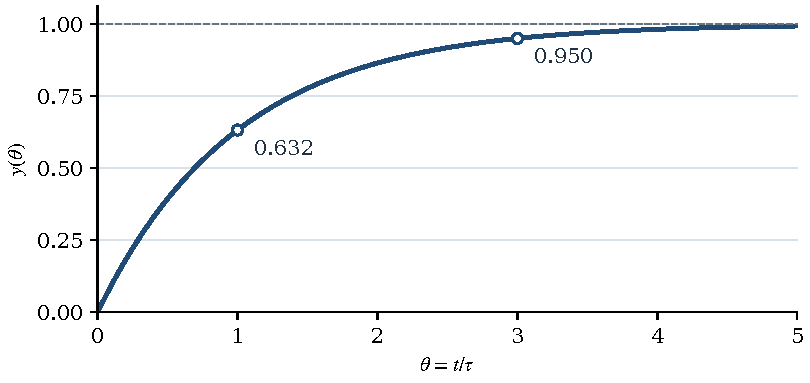
\includegraphics[width=0.76\linewidth]{figures/step-response.pdf}
  \caption{单位阶跃输入下的一阶系统归一化响应}
  \label{fig:step-response}
\end{figure}

\subsection{固定时刻比较}

表~\ref{tab:time-constants} 给出在同一时刻的计算值。$\tau$ 从 \qty{0.5}{\second} 增至 \qty{2.0}{\second} 时，输出从约 $0.982$ 降至 $0.632$。这是因为更大的时间常数对应更小的 $t/\tau$，而不是因为系统稳态增益变小。

% 表题在表上，表注在表底线下；S 列按小数点对齐。
\begin{table}[htbp]
  \centering
  \caption{不同时间常数下的固定时刻响应}
  \label{tab:time-constants}
  \begin{tabular}{@{}l S[table-format=1.1] S[table-format=1.1] S[table-format=1.3]@{}}
    \toprule
    工况 & {$\tau/\unit{\second}$} & {$t/\tau$} & {$y(t)$} \\
    \midrule
    较快 & 0.5 & 4.0 & 0.982 \\
    基准 & 1.0 & 2.0 & 0.865 \\
    较慢 & 2.0 & 1.0 & 0.632 \\
    \bottomrule
    \multicolumn{4}{@{}l@{}}{\zihao{5} 注：取 $t=\qty{2}{\second}$，输出保留三位小数。}
  \end{tabular}
\end{table}

\section{结论}

在单位增益和零初始状态下，一阶阶跃响应可由 $t/\tau$ 统一描述：一个时间常数约达到稳态值的 \qty{63.2}{\percent}，三个时间常数约达到 \qty{95.0}{\percent}。固定时刻比较时，时间常数越小，越接近稳态。若将此方法用于实际设备，应先判断纯滞后和高阶动态是否可忽略，再用测量数据验证模型。


\printbibliography[title={参考文献}]
\end{document}
